% Compile with: lualatex presentation.tex
% Then for SVG: dvisvgm --zoom=-1 --exact --page=1,- --font-format=woff2 presentation.dvi
% Or just: latexmk -pdf presentation.tex for PDF only

\documentclass[aspectratio=169, 14pt, t]{beamer}

% Packages
\usepackage[utf8]{inputenc}
\usepackage[T1]{fontenc}
\usepackage{helvet}
\usepackage{amsmath}
\usepackage{amssymb}
\usepackage{graphicx}
\usepackage{physics}
\usepackage[absolute,overlay]{textpos}
\usepackage{tikz}
\usepackage{tikz-3dplot}

% Font setup
\renewcommand{\familydefault}{\sfdefault}

% Colors - Clean minimal palette
\definecolor{slidetext}{RGB}{60,64,67}
\definecolor{slidetitle}{RGB}{0,0,0}
\definecolor{authortext}{RGB}{120,120,120}
\definecolor{fieldblue}{RGB}{70,130,180}
\definecolor{electronred}{RGB}{200,60,60}

\setbeamercolor{normal text}{fg=slidetext}
\setbeamercolor{frametitle}{fg=slidetitle}
\setbeamercolor{title}{fg=slidetitle}
\setbeamercolor{background canvas}{bg=white}
\setbeamercolor{itemize item}{fg=slidetext}

% Font Sizes
\setbeamerfont{title}{size=\fontsize{36}{44}\selectfont}
\setbeamerfont{frametitle}{size=\fontsize{25}{30}\selectfont}
\setbeamerfont{normal text}{size=\fontsize{18}{24}\selectfont}
\setbeamerfont{author}{size=\fontsize{8}{10}\selectfont}

% Clean Layout
\setbeamertemplate{navigation symbols}{}
\setbeamertemplate{headline}{}

% Title Page with TikZ illustration
\setbeamertemplate{title page}{
    \begin{centering}
        \usebeamerfont{title}\color{black}
        Quantum Motion in a \\
        Uniform Magnetic Field
        \par
    \end{centering}
    % TikZ illustration - electron spiral in B-field
    \begin{textblock*}{6cm}(7cm, 5.5cm)
        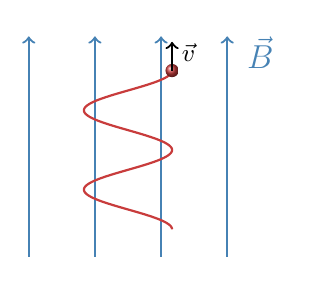
\begin{tikzpicture}[scale=0.7]
            % Magnetic field arrows (vertical)
            \foreach \x in {0, 1.2, 2.4, 3.6} {
                \draw[->, thick, fieldblue] (\x, -0.5) -- (\x, 3.5);
            }
            % B label
            \node[fieldblue, font=\large] at (4.2, 3.2) {$\vec{B}$};
            
            % Electron spiral path
            \draw[thick, electronred, domain=0:720, samples=200, smooth] 
                plot ({1.8 + 0.8*cos(\x)}, {0.004*\x});
            
            % Electron
            \shade[ball color=electronred] (1.8+0.8, 2.88) circle (0.12);
            \node[electronred, font=\small] at (3.2, 2.88) {};
            
            % Velocity arrow
            \draw[->, thick, black] (2.6, 2.88) -- (2.6, 3.4);
            \node[font=\small] at (2.9, 3.2) {$\vec{v}$};
        \end{tikzpicture}
    \end{textblock*}
    \begin{textblock*}{5cm}(10.9cm, 8.2cm)
        \begin{flushright}
            \usebeamerfont{author}\color{authortext}
            Ali EL AZDI (IN BA5)
        \end{flushright}
    \end{textblock*}
}

% Frame Title
\setbeamertemplate{frametitle}{
    \vskip0.3cm
    \insertframetitle
    \vskip0.2cm
}

% Bullets
\setbeamertemplate{itemize item}{\small\raise0.5pt\hbox{\textbullet}}
\setbeamertemplate{itemize subitem}{\small\raise0.5pt\hbox{\textbullet}}

% Metadata
\title{Quantum Motion in a Uniform Magnetic Field}
\author{Ali EL AZDI (IN BA5)}
\date{\today}

\begin{document}

% Slide 1: Title
\begin{frame}[plain,c]
    \titlepage
\end{frame}

% Slide 2: Why?
\begin{frame}{Why study this problem?}
    \vspace{0.5cm}
    \begin{itemize}
        \item \textbf{Theoretical Foundation}: One of the few exactly solvable interactions in Quantum Mechanics
        \item \textbf{Condensed Matter}: Describes electrons in metals and semiconductors (2D electron gas)
        \item \textbf{Quantum Hall Effect}: Explains macroscopic quantum phenomena and resistance standards
    \end{itemize}
\end{frame}

% Slide 3: Lorentz Force
\begin{frame}{Background: What we need to know}
    A particle with charge $q$ moving at velocity $\vec{v}$ in an electromagnetic field is subject to the general \underline{\textbf{Lorentz Force}}:
    \vfill
    \[
        \vec{F} = q(\vec{E} + \vec{v} \times \vec{B})
    \]\vfill
    $E$ the electric field, $B$ the magnetic field, $q$ the charge of the particle and $\vec{v}$ the velocity of the particle.
\end{frame}

% Slide 4a: Visualization Setup
\begin{frame}{Example: Classical Motion}
    \textbf{Setup Conditions:}
    \vspace{0.5cm}
    \begin{itemize}
        \item \textbf{System:} Particle $q < 0$ confined to $xy$-plane
        \item \textbf{Field:} Static uniform $\vec{B} = B\hat{z}$ ($E=\frac{dB}{dt} = 0$)
        \item \textbf{Motion:} Cyclotron orbit $r = \frac{mv}{|q|B}$
    \end{itemize}
\end{frame}

% Slide 4: Visualization (placeholder for video in HTML)
\begin{frame}{Example: Classical Motion}
    \begin{center}
       
    \end{center}
\end{frame}

% Slide 5: The Question
\begin{frame}{}
    \vfill
    \begin{center}
        \large
        \textit{What are the quantum energy levels of a}\\
        \textit{charged particle in a uniform magnetic field?}
    \end{center}
\end{frame}

% Slide 5: The Vector Potential
\begin{frame}{The Vector Potential}
    Since $\nabla \cdot \vec{B} = 0$, we can write: $\vec{B} = \nabla \times \vec{A}$ \\[0.5cm]
    \textbf{Gauge Freedom}: $\vec{A}$ is not unique $ \vec{A}' = \vec{A} + \nabla\chi $. \\[0.5cm]
    We choose the  \underline{\textbf{Landau Gauge}} for $\vec{B} = B\hat{z}$:
    \[ \vec{A} = (0, Bx, 0) \]
\end{frame}

% Slide 5b: Classical Hamiltonian
\begin{frame}{Deriving the Classical Hamiltonian}
    \textbf{Energy and Momentum}
    \begin{itemize}
        \item Total Energy: $E_{total} = \frac{1}{2}m\vec{v}^2 + q\phi$
        \item Canonical Momentum: $\vec{p} = m\vec{v} + q\vec{A}$
    \end{itemize}
    \vspace{0.5cm}
    \[
        H = \frac{1}{2m}(\vec{p} - q\vec{A})^2 + q\phi
    \]
    \vfill
    \textbf{Verification:} Hamilton's equations recover the Lorentz force:
    \[ \dot{\vec{r}} = \nabla_{\vec{p}} H \qc \dot{\vec{p}} = -\nabla_{\vec{r}} H \]
\end{frame}


\begin{frame}{Quantum Mechanics Setup}
    \textbf{Canonical Quantization}: promote variables to operators.
    \begin{itemize}
        \item Position: $\vec{r} \to \hat{\vec{r}}$
        \item Momentum: $\vec{p} \to \hat{\vec{p}} = -i\hbar\nabla$
    \end{itemize}
    
    \vspace{0.5cm}
    Substitute into Classical Hamiltonian:
    \[ H = \frac{1}{2m}(\vec{p} - q\vec{A})^2 \quad \longrightarrow \quad \hat{H} = \frac{1}{2m}(\hat{\vec{p}} - q\vec{A}(\hat{\vec{r}}))^2 \]
\end{frame}
% Slide 7: Hamiltonian under Landau Gauge
\begin{frame}{Hamiltonian under Landau Gauge}
    \begin{itemize}
        \item Schrödinger Equation: $\hat{H}\ket{\psi} = E\ket{\psi}$
    \end{itemize}\vspace{0.5cm}
    Using $\vec{A} = (0, Bx, 0)$:
    \[
        \hat{H} = \frac{1}{2m}\left[ \hat{p}_x^2 + (\hat{p}_y - qBx)^2 + \hat{p}_z^2 \right]
    \]
    The Schrödinger equation becomes:
    \[
        \frac{1}{2m}\left[ \hat{p}_x^2 + (\hat{p}_y - qBx)^2 + \hat{p}_z^2 \right] \psi = E\psi
    \]
\end{frame}

% Slide 8: Solving the Equation
\begin{frame}{Solving the Equation}
    Since $\hat{H}$ is independent of $y$ and $z$, \\$p_y = \hbar k_y$, $p_z = \hbar k_z$ are conserved.\\[0.1cm]
    \begin{minipage}[t]{0.62\textwidth}Ansatz:
    \[ \psi(\vec{r}) = e^{i(k_y y + k_z z)} \phi(x) \]
    \end{minipage}\hfill\vline\hfill
    \begin{minipage}[t]{0.34\textwidth}
        \small
        \textbf{Definitions}\\[0.2cm]
        $\omega_c = \dfrac{|q|B}{m}$\\[0.2cm]
        $x_0 = \dfrac{\hbar k_y}{qB}$
    \end{minipage}\\[0.1cm]
    This reduces the problem to 1D:
    \[
        \left[ \frac{\hat{p}_x^2}{2m} + \frac{1}{2}m\omega_c^2(x - x_0)^2 \right]\phi(x) = \left(E - \frac{\hbar^2 k_z^2}{2m}\right) \phi(x)
    \]
    \vspace{0.5cm}
\end{frame}

% Slide 9: Landau Levels
\begin{frame}{Result: Landau Levels}
    We recognize a \textbf{Harmonic Oscillator's} Hamiltonian!
    
    \vspace{1cm}
    Energy eigenvalues:
    \[
        E_{n, k_z} = \hbar\omega_c\left(n + \frac{1}{2}\right) + \frac{\hbar^2 k_z^2}{2m}
    \]
    for $n = 0, 1, 2, \dots$
    
    \vspace{0.5cm}
    \begin{itemize}
        \item $n$ is the harmonic oscillator's excitation level, quantized cyclotron orbits (\textbf{Landau Levels})
    \end{itemize}
\end{frame}

% Slide 10: Energy Level Comparison
\begin{frame}{Energy Levels}
    
    \begin{minipage}[t]{0.48\textwidth}
        \centering
        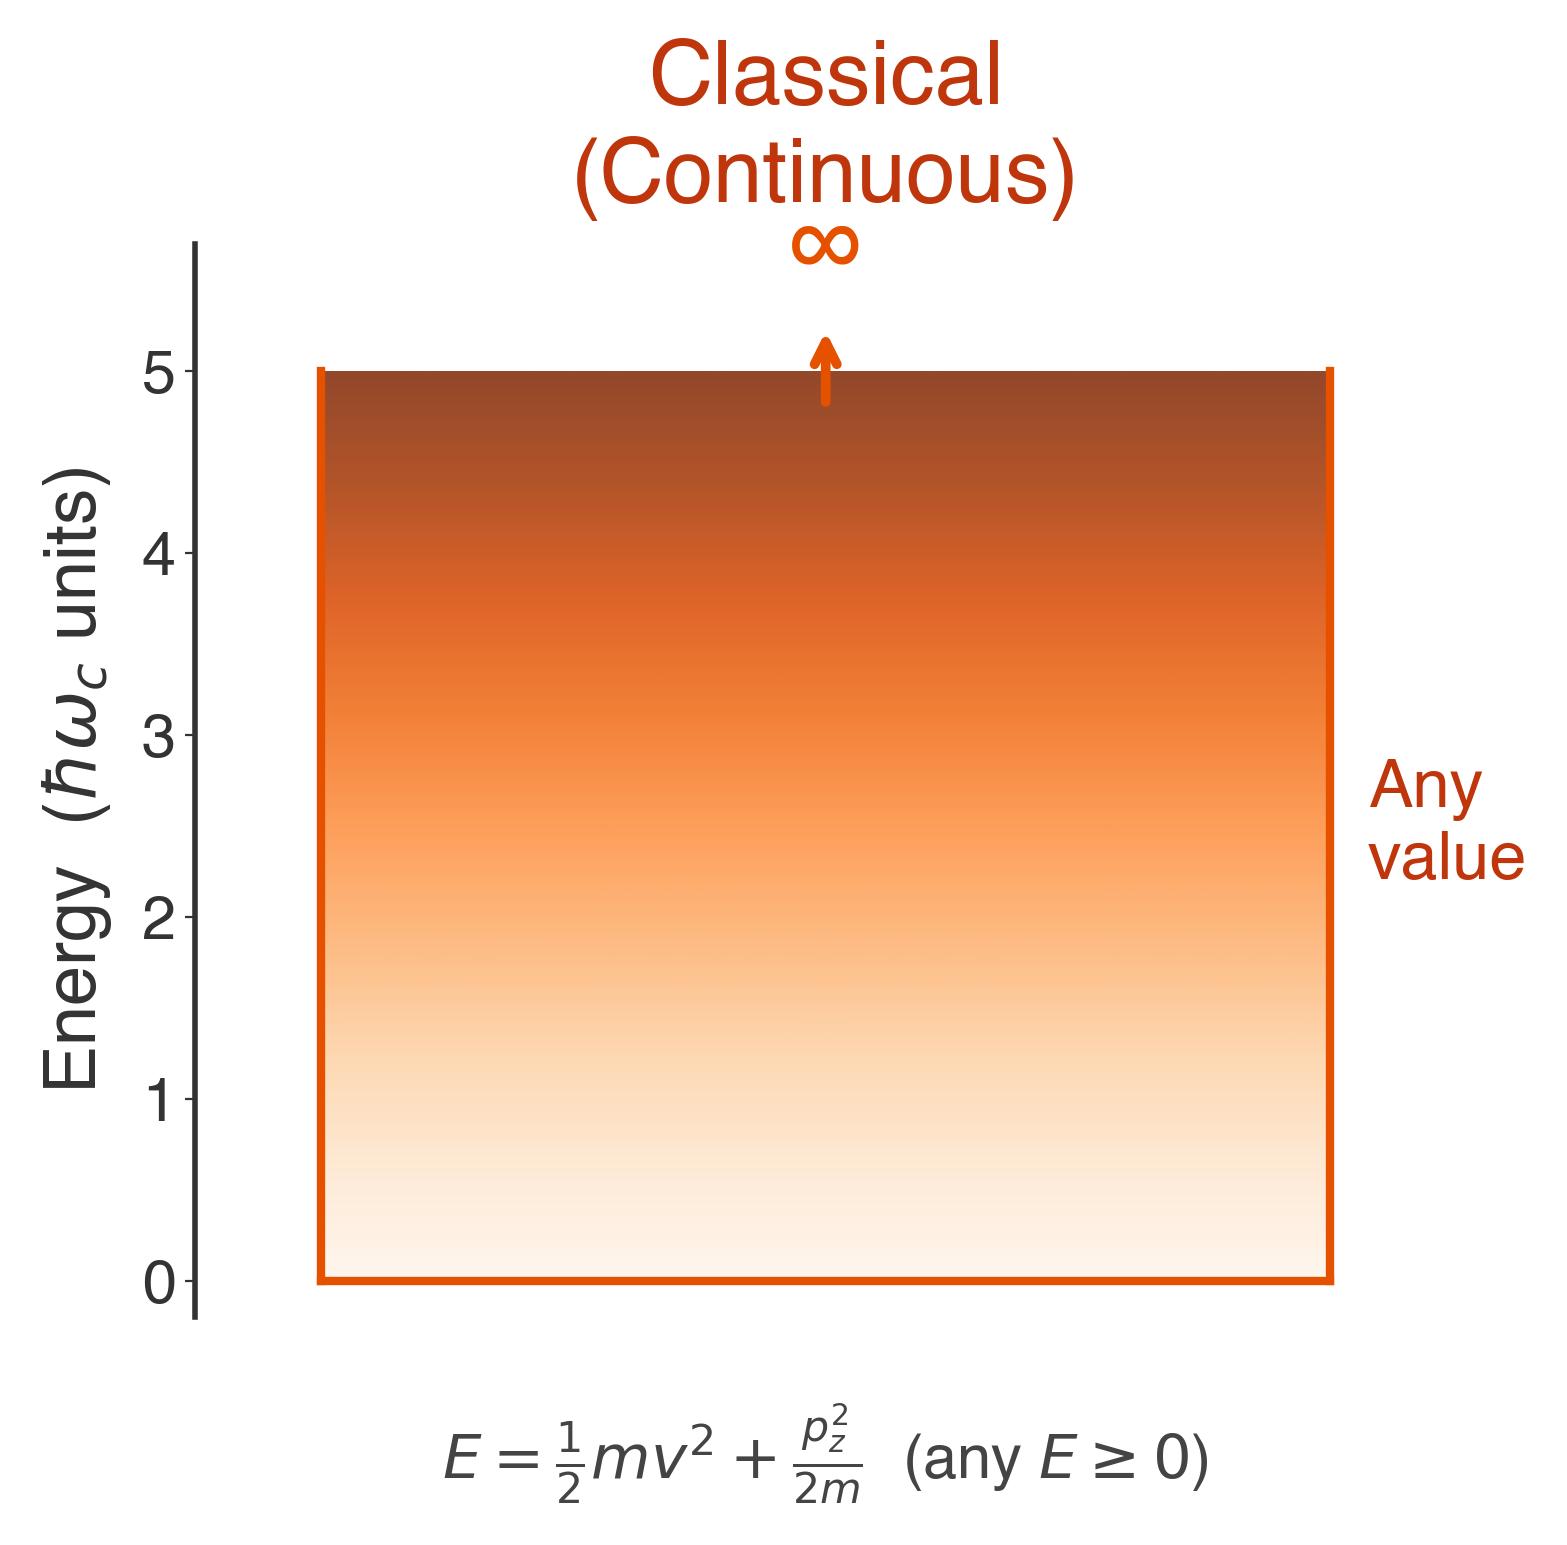
\includegraphics[width=1.03\textwidth]{media/classical_energy_levels.png}
    \end{minipage}\hfill\vline\hfill
    \begin{minipage}[t]{0.48\textwidth}
        \centering
        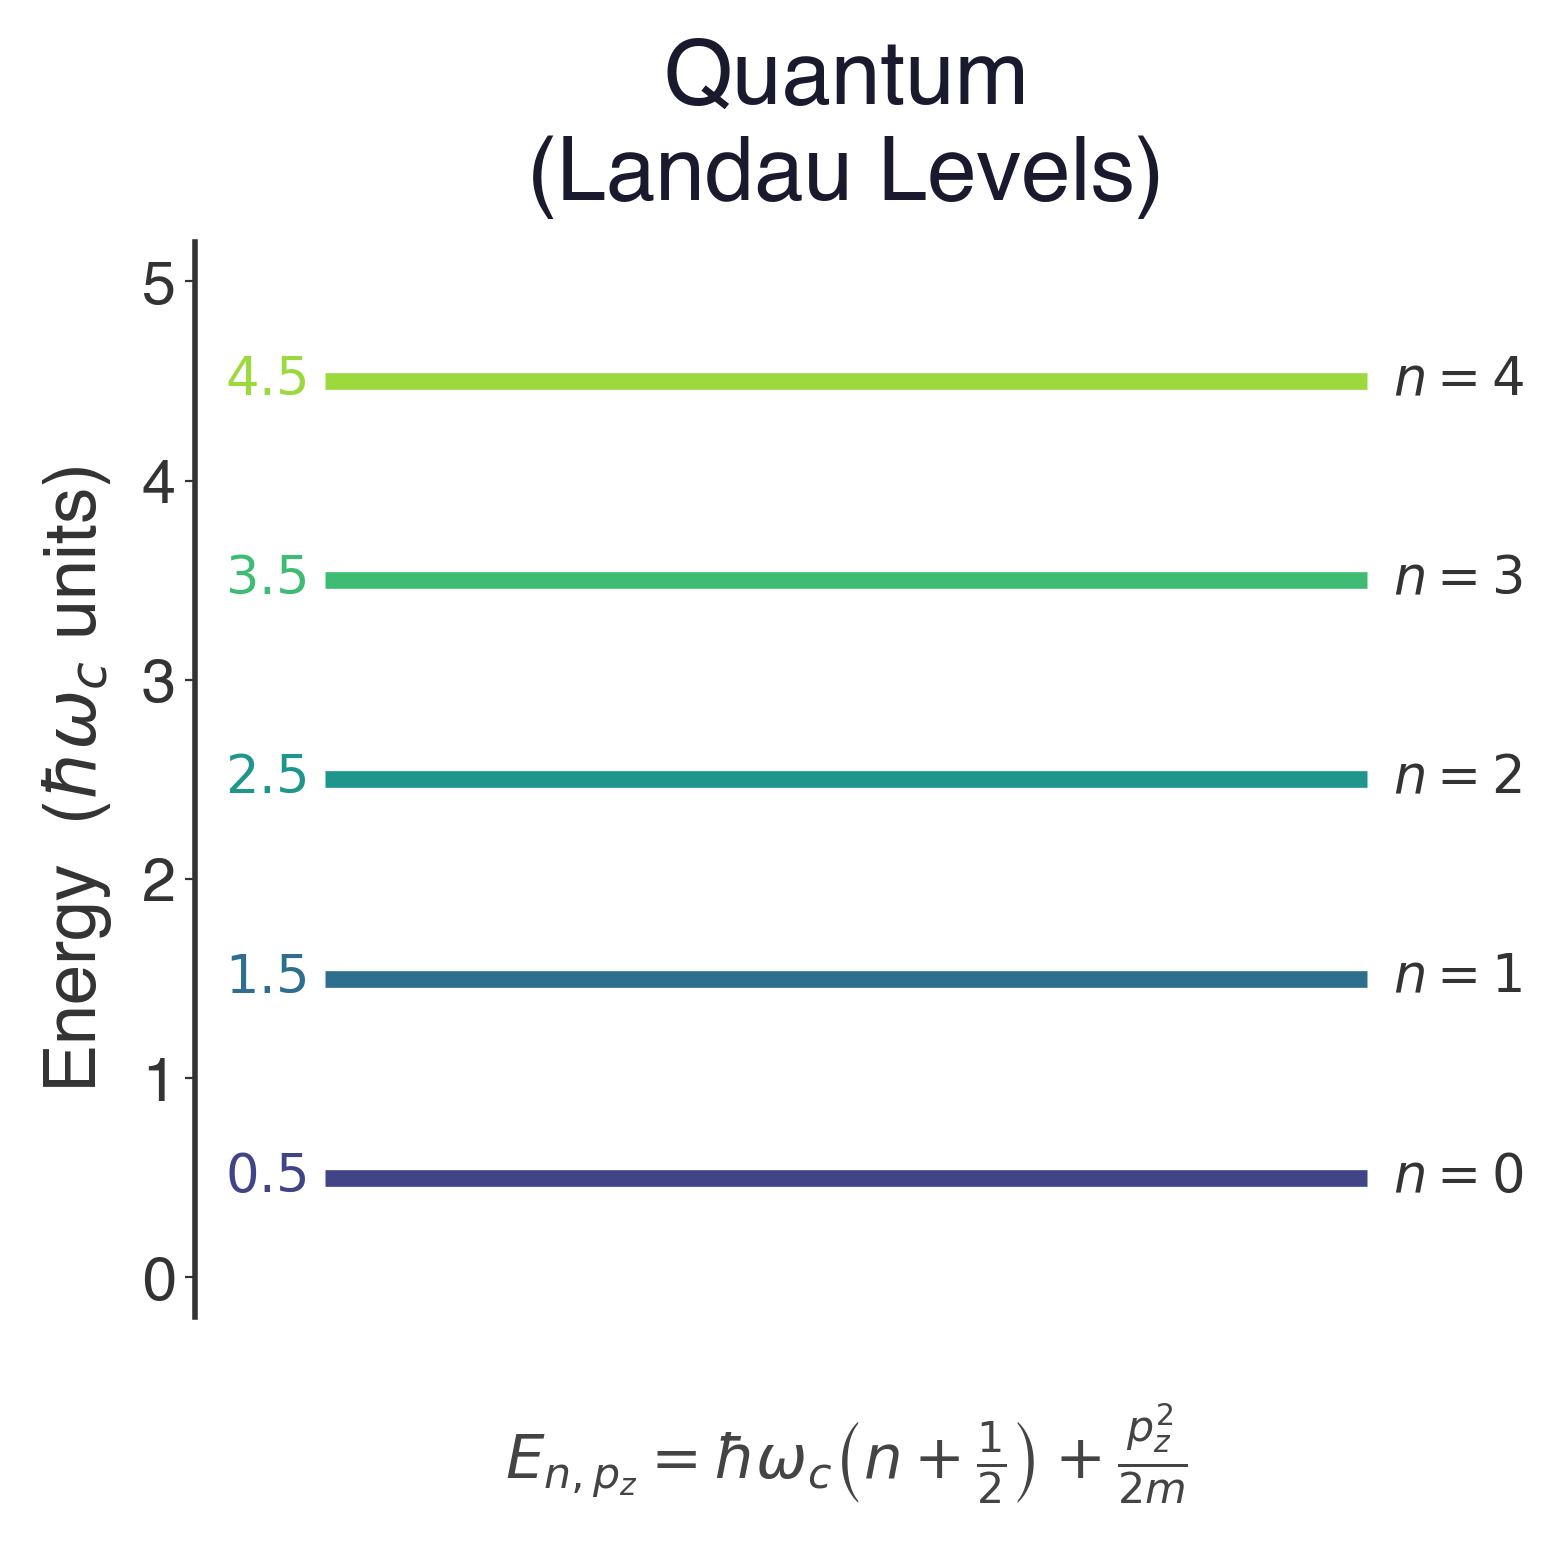
\includegraphics[width=1.03\textwidth]{media/quantum_energy_levels.png}
    \end{minipage}
\end{frame}

% Slide 11: Wavefunction Visualization
\begin{frame}{The Complete Wavefunction}
    \begin{itemize}
        \item Center of oscillation $x_0 = \frac{\hbar k_y}{qB}$ depends on wavenumber $k_y$
        \item $\phi_n$ is the harmonic oscillator wavefunction
    \end{itemize}
    \vfill
    Full solution:
    \[
        \psi_{n,k_y,k_z}(x,y,z) = e^{i(k_y y + k_z z)} \cdot \phi_n(x - x_0)
    \]
    \vfill
    Different $k_y$ values give same energy $\rightarrow$ \textbf{degeneracy}
\end{frame}


% Auxiliary 2: Degeneracy
\begin{frame}{Landau Level Degeneracy}
    The energy $E_n$ does not depend on $k_y$ (or $x_0$).
    \vspace{0.5cm}
    
    For a sample of area $A = L_x \times L_y$:
    \[
        N = \frac{|q|B A}{h} = \frac{\Phi}{\Phi_0}
    \]
    \vspace{0.3cm}
    \begin{itemize}
        \item $\Phi = BA$ = total magnetic flux
        \item $\Phi_0 = h/|q|$ = flux quantum
        \item Degeneracy $\propto$ magnetic field strength
    \end{itemize}
\end{frame}

% Auxiliary 3: Example
\begin{frame}{Example: Magnitude of Degeneracy}
    Consider a sample of size $1\,\text{cm} \times 1\,\text{cm}$ in a field $B = 1.5\,\text{T}$ (typical MRI).
    \vspace{0.3cm}
    
    The degeneracy is:
    \[
        N = \frac{|q|B A}{h} = \frac{(1.6 \times 10^{-19})(1.5)(10^{-4})}{6.63 \times 10^{-34}} \approx 3.6 \times 10^{10}
    \]
    \vspace{0.3cm}
    \begin{itemize}
        \item About \textbf{36 billion states} in each Landau level!
        \item Huge degeneracy $\rightarrow$ Quantum Hall Effect
    \end{itemize}
\end{frame}


% Slide 12: References
\begin{frame}{References}
    \begin{itemize}
        \normalsize
        \item \textbf{MIT L14.3 Particle in a constant magnetic field: Landau Levels} \\
        \small \url{https://www.youtube.com/watch?v=Uux0VkKaoxY&t=18s}
        \vspace{0.2cm}
        \normalsize
        \item \textbf{Lecture 5: Motion of a charged particle in a magnetic field} \\
        \small \url{http://www.tcm.phy.cam.ac.uk/~bds10/aqp/lec5_compressed.pdf}
    \end{itemize}
\end{frame}

%%%%%%%%%%%%%%%%%%%%%%%%%%%%%%%%%%%%%%%%%%%%%%%%%%%%%%%%%
% AUXILIARY SLIDES (for Q&A)
%%%%%%%%%%%%%%%%%%%%%%%%%%%%%%%%%%%%%%%%%%%%%%%%%%%%%%%%%

\appendix

% Auxiliary 1: Why Landau Gauge?
\begin{frame}{Auxiliary: Why the Landau Gauge?}
    Two common gauge choices for $\vec{B} = B\hat{z}$:
    \vspace{0.3cm}
    \begin{itemize}
        \item \textbf{Landau Gauge}: $\vec{A} = (0, Bx, 0)$
        \begin{itemize}
            \item Breaks rotational symmetry
            \item Leads to Cartesian separable solution
        \end{itemize}
        \item \textbf{Symmetric Gauge}: $\vec{A} = \frac{B}{2}(-y, x, 0)$
        \begin{itemize}
            \item Preserves rotational symmetry
            \item Leads to solutions in polar coordinates
        \end{itemize}
    \end{itemize}
    \vspace{0.5cm}
    Both give the \textit{same physics} (same energy levels, same observables).
\end{frame}

% Auxiliary 2: Estimating Magnetic Length
\begin{frame}{Auxiliary: Magnetic Length 1}
    The magnetic length $\ell_B$ arises naturally from the harmonic oscillator analogy.
    \vspace{0.3cm}
    characteristic length of a harmonic oscillator:
    \[ l = \sqrt{\frac{\hbar}{m\omega}} \]
    
    Substitute the cyclotron frequency $\omega \to \omega_c = \frac{|q|B}{m}$:
    \[
        \ell_B = \sqrt{\frac{\hbar}{m\omega_c}} = \sqrt{\frac{\hbar}{m\left(\frac{|q|B}{m}\right)}} = \sqrt{\frac{\hbar}{|q|B}}
    \]
\end{frame}

\begin{frame}{Auxiliary: Magnetic Length 2}
    \textbf{Question}: How small is $\ell_B$ in practice?
    \vspace{0.3cm}

    \textbf{Example}: For a strong field $B = 1.5\,\text{T}$ (MRI):
    \[
        \ell_B \approx \sqrt{\frac{1.055 \times 10^{-34}}{1.6 \times 10^{-19} \times 1.5}} \approx 21\,\text{nm}
    \]
    \vspace{0.3cm}
    \textbf{Physical Meaning}:
    \begin{itemize}
        \item Defines the size of the electron's wavefunction
        \item Area per quantum state: $A_{\text{state}} \approx 2\pi\ell_B^2$
    \end{itemize}
\end{frame}


% Auxiliary 3: Quantum Hall Effect
\begin{frame}{Auxiliary: Quantum Hall Effect}
    When Landau levels are filled:
    \[
        \sigma_{xy} = \nu \frac{e^2}{h}
    \]
    \vspace{0.3cm}
    \begin{itemize}
        \item $\nu$ = number of filled Landau levels
        \item $R_K = h/e^2 \approx 25.8\,\text{k}\Omega$ = von Klitzing constant
        \item Used as resistance standard (Nobel Prize 1985)
    \end{itemize}
\end{frame}

\end{document}
